\section{Enhancements}

In this section we will discuss about all the necessary enhancements and amendments done to the data flow values 
(refer Fig ~\ref{fig:Data Flow Equations}). Those mainly involve corrections, tackling unhandled cases and augmentations
to make the analysis more precise.

\textbf{Correctness}:
Lets discuss a scenario which involve correctness issue.

{\small \tt
\begin{center}
    \begin{tabular}[b]{l}
      S1. l$\rightarrow$f = m; \\
      S2. m$\rightarrow$f = l; \\
      S3. l = null;
    \end{tabular}
\end{center}
  }

\begin{example}
Consider the sample code given above. After statement {\tt S1} there is a path from {\tt l} to {\tt m} via field {\tt f} and 
after {\tt S2} there is a path from {\tt m} to {\tt l} also via field {\tt f} hence creating a cycle.
When {\tt S3} is done there is still a cycle at {\tt m}. The relevant Direction matrix entries after {\tt S2} are: 
\begin{eqnarray*}
\mbox{After {\tt S1} : }  D_{F}[l,m] &=& \fieldD{f}{} , f_{l,m} = 1  \\
\mbox{After {\tt S2} : }    D_F[l,m] &=& \fieldD{f}{} , D_F[m,l] = \fieldD{f}{} , \f_{l,m} = 1 , \f_{m,l} = 1  
\end{eqnarray*}
The boolean equation of $l_{\subC}$ after {\tt S2} is 
\[
\{ \f_{l,m} \wedge ( \num{D_F[m,l]} >= 1) \} \vee \{  (\f_{m,l} \wedge   ( \num{D_F[l,m]} >= 1)) \}   
\]
which evaluates to true assuring that there is a cycle at {\tt l} after {\tt S2}. After statement {\tt S3} all the Direction and 
Interference information corresponding to {\tt l} are killed, i.e. 
$D_F[l,m]= \emptyset , D_F[m,l]= \emptyset , \f_{l,m}=0 , \f_{m,l}=0.$ 

As a result  ${\tt l}_{\subC}$ gets evaluated to 0 inferring it is not a CYCLE, which is not true.
\end{example}      

\textbf{Solution:} The problem is, after statement {\tt S3} we are killing all the information related to pointer variable {\tt l}
even though the graph structure still contains the corresponding heap object. We need to somehow preserve the information about the node 
which is labeled with name {\tt l} before {\tt S3} and unlabeled afterwards.

For this we create a new dummy pointer variable (say $\delta$) pointing to the same node pointed by {\tt l} before {\tt S3}.
This is done by adding a statement $\delta = l$ before {\tt S3} such that this particular statement will not be having
any kill information. The GEN information will be same as the pointer statement {\tt p = q}. Also we replace any information about the term 
l by $\delta$, i.e.\ in the $D_F$, $I_F$ matrices and in all the boolean equations corresponding to all the heap pointers, we replace 
the occurrences of l by  $\delta$.
So the solution can be generalized as:

Whenever any statement of type \textit{Allocations} or \textit{Pointer Assignments} are encountered, we add a new statement
$\delta = \p$ before it where $\delta$ is a dummy variable of same type as \p. For this new statement 
we have the following gen and kill relations.

\begin{center}
$\GenC{\delta}   = \InC{\p}[\p/\delta] \quad \GenD{\delta} = \InD{\p}[\p/\delta]$ \\
\end{center}
$\forall \s \in \heap, \s \not= \p, \forall f \in \fields$ 
\begin{center}
$\KillC{\s}   = \InC{\s}  \ \ \KillD{\s} = \InD{\s}$  \\
$\GenC{\s}   = \InC{\s}[\p/\delta] \ \  \GenD{\s} = \InD{\s}[\p/\delta]$ \\ 	 
\end{center}

      
	\textit{where $X[\q / \p]$ creates a copy of $X$ with all occurrences
	of $\q$ replaced by $\p$.}

$\forall \s \in \heap, \s \not= \p, \forall f \in \fields$ 

\begin{center}
\begin{tabular}{cc}
$f_{\delta\s} = f_{\p\s}$  &  $f_{\s\delta} = f_{\s\p}$ \\

$D_F^{\dgen}[\delta,\s]$    =  $D_F^{\din}[\p,\s]$ &  $D_F^{\dgen}[\s,\delta]$    =  $D_F^{\din}[\s,\p]$   \\

$D_F^{\dgen}[\delta,\delta]$    =  $D_F^{\din}[\p,\p]$  &  $I_F^{\dgen}[\delta,\s]$    =   $I_F^{\din}[\p,\s]$ \\

$I_F^{\dgen}[\delta,\delta]$    = $I_F^{\din}[\p,\p]$  \\
\end{tabular}
\end{center}

We have two options in adding the new statement {\tt $\delta$ = p}: Use the same dummy $\delta$ variable every time or
 use different dummy variables for each new statement added. Now if we use the same variable then at some point different unlabeled nodes will be 
 using the same name $\delta$ causing less precise results. We can also use new variable every time for more precise results, but 
 this will increase memory consumption. So usage of a single variable or multiple variables is a matter of trade off between 
 accuracy and memory consumption. As this statement doesn't have any kill information, it may happen at some point that this pointer is referring to a
summarized node which indeed contains distinct nodes. This can have an effect on preciseness, details about its effect are given in the Results Chapter.\\ \\
\textbf{Unhandled Dataflow Information}:
Before we go into this we need to understand what does  $\epsilon \in D_F^{\din}[\p,\q]$ convey. It means that we can reach q from p through
the path Epsilon, which simply says \p\ and \q\ are pointing to the same heap object, i.e.\ they both are aliases. Some of the data flow information
present in Fig:~\ref{fig:Data Flow Equations} (shaded with blue) didn't consider the effect on aliases, and so we considered those as well.

\begin{itemize}
\item{\tt p $\rightarrow$ f = NULL}	: 

We can see that the equation $D_F^{\dkill}[\s,\q] = \emptyset$ doesn't consider the case when s and p are aliases,
in that case $D_F^{\dkill}[\s,\q]$ should be equal to $\project{D_F^{\din}[\s,\q]}{f}$, which is similar what $D_F^{\dkill}[\p,\q]$ is assigned.
A similar modification is also required for the equation $I_F^{\dkill}[\q,\s] = \emptyset$ when p and q are aliases. In that case we have
 $I_F^{\dkill}[\q,\s] = \{(\alpha, \beta) \ \vert\ (\alpha,   \beta) \in I_F^{\din}[\q, \s] \mbox,\ \alpha \equiv  f^\anysup \ \}$, otherwise
 the original equation holds good. We fine tune all the data flow values so as to incorporate the such effects of aliases in our analysis (refer Fig:~\ref{fig:Modified Data Flow Equations} ).
Now consider a scenario that there is a self loop at \p\ so that the entry $I_F^{\dkill}[\p,\p]$ will contain something like $\{ \fieldD{f}{} ,\epsilon \}$ 
which indeed should be killed once this statement is encountered. So we write 
$I_F^{\dkill}[\p,\p] = \{(\alpha, \beta) \ \vert\ (\alpha,   \beta) \in I_F^{\din}[\p, \p] \mbox,\ \alpha \equiv  f^\anysup \ \}$. 

%This amonts to the following addition:

%$I_F^{\dkill}[\myr,\myr] = \left\{\begin{array}{@{}ll}
%%	  \{(\alpha, \beta) \ \vert\ (\alpha,   \beta) \in I_F^{\din}[\myr, \myr] \mbox,\ \alpha \equiv  f^\anysup \ \} &  \epsilon \in D_F^{\din}[\p,\myr] \vee  \myr=\p \\
%	  \emptyset & \mbox{Otherwise}                            
%	  \end{array}\right.$ \\
           
\item{\tt p $\rightarrow$ f = q}:

%Kill info is same as that of {\tt p $\rightarrow$ f = NULL}, so the above modifications holds good here too.

\begin{figure}[h]
\begin{center}
\begin{tabular}{c}

%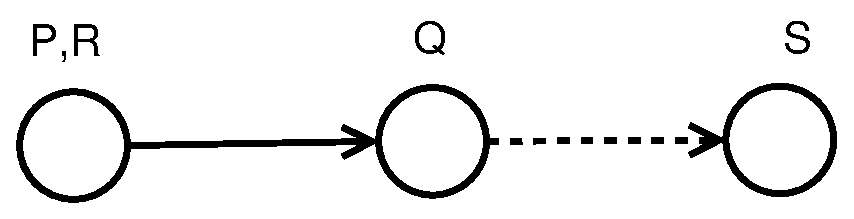
\includegraphics[scale=.4]{diagrams/Impl_1.eps} 
%&
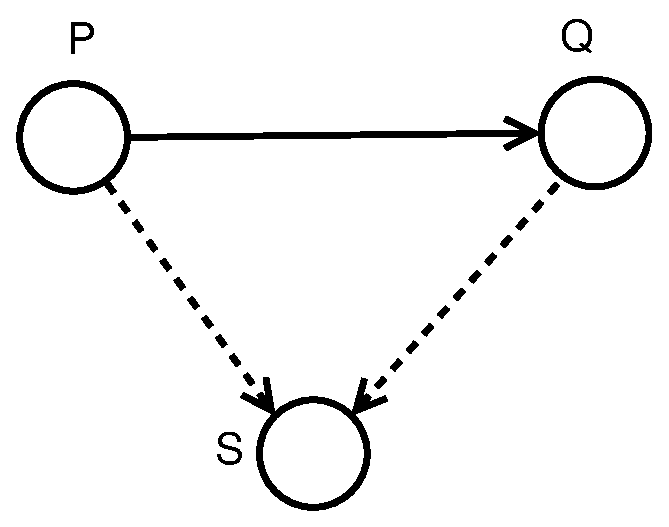
\includegraphics[scale=.4]{diagrams/Impl_2.eps} %& 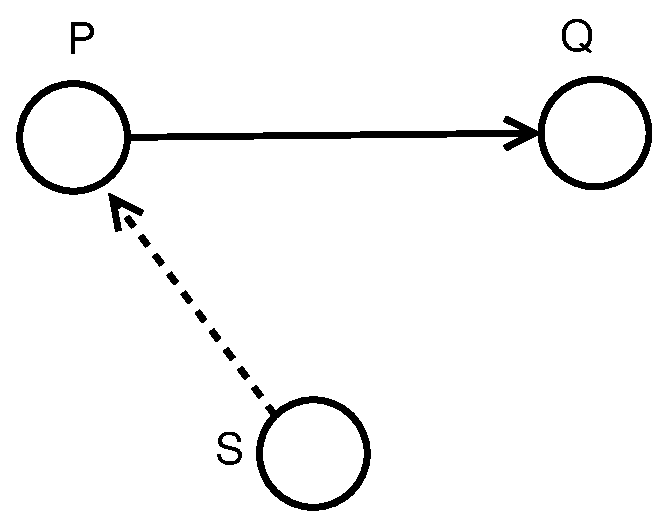
\includegraphics[scale=.4]{diagrams/Impl_3.eps} \\
 %\footnotesize (a) %& \footnotesize (b) 
\end{tabular}
\caption{Heap graphs}  \label{fig:Eq5_example}
\end{center}
\end{figure}

%Consider the assignment of $D_F^{\dgen}[\myr,\s]$ where $\s \not= \p,\ \myr \not\in   \{\p, \q\}$ .What if $\myr$  and $\p$ are aliases then it would 
%be equal to $\num{D_F^{\din}[\q, \s]} \star \epsilonset$ giving incorrect information although there is a path via field $\f$ to $\s$.Fig:~\ref{fig:Eq5_example}(a)
%gives us a picture of how it is.Hence when $\myr$ and $\p$ are aliases  $D_F^{\dgen}[\myr,\s]$ is assigned to $\num{D_F^{\din}[\q, \s]} \star \fieldI{f}{}{1}$.Hence
%its modified as 
%
%
%
%
%
%$D_F^{\dgen}[\myr, \s] = \left\{\begin{array}{@{}ll}
%\num{D_F^{\din}[\q, \s]} \star \fieldI{f}{}{1} & \epsilon \in D_F^{\din}[\myr,\p]  \\
%\num{D_F^{\din}[\q, \s]} \star
%D_F^{\din}[\myr, \p] & \mbox{Otherwise}
%%\end{array}\right.$  $\s \not= \p,\ \myr \not\in \{\p, \q\}$ \\
%
%
%    
%    \quad \quad  For the data flow equation of $I_F^{\dgen}[\p, \q]$ there are two modifications.For the first one assume a self loop is present at $\p$ through field $\f$ .
%And a statement of form $\p \rightarrow \f = \myr$ is encountered.Then according to the previous version of this data flow equation $I_F^{\dgen}[\p, \myr]$ would be
%$\{(\fieldD{f}{}, \epsilon)\} \cup ( \fieldI{f}{}{1} \times \epsilonset)$ ,because of which we wrongly infer that there are two paths through which $\p$ and $\myr$
%intersect.This information at some cases can make our analysis conservative by reporting p as a DAG even though its a TREE.For this reason we modify the equations as
%$\{(\fieldD{f}{}, \epsilon)\}
%  \cup ((1 \star (\remOne{D_F^{\din}[\p,
%      \p]}{ \{\project{D_F^{\din}[\p,\p]}{f} \cup \epsilonset \} })) \times \epsilonset)$ \\



Consider the heap graph in Fig:~\ref{fig:Eq5_example}, you can notice that the heap nodes pointed by $\p$ and $\q$ interfere at $\q$ as well as
at $\s$. The latter part is not captured by  $I_F^{\dgen}[\p, \q]$ i.e 

$I_F^{\dgen}[\p, \q]$ = $\{(\fieldD{f}{}, \epsilon)\}
  \cup ((1 \star (\remOne{D_F^{\din}[\p,
      \p]}{ \{\project{D_F^{\din}[\p,\p]}{f} \cup \epsilonset \} })) \times \epsilonset)$

This equation is not considering the effect when both $\p$ and $\q$ reach some node pointed by $\s$ at which they interfere. 
To handle this case we look at the  set of all heap pointer's $\s$ which is not equal to $\p$ or $\q$ but has paths to it from $\p$ and $\q$.
Going by the definition of Interference matrix we find the fields through which these two pointers interfere, which is nothing but
$D_F^{\din}[\p,\s] \times D_F^{\din}[\q,\s]$. The Union of all such elements for each $\s$ constitute our final information. Thus

  $\{(\fieldD{f}{}, \epsilon)\}
  \cup ((1 \star (\remOne{D_F^{\din}[\p,
      \p]}{ \{\project{D_F^{\din}[\p,\p]}{f} \cup \epsilonset \} })) \times \epsilonset) \cup  \I$ \\
  \quad \quad where \ 
  $\I  =   \bigcup_{s\in\heap,\s \not= \p,\q } \{ {D_F^{\din}[\p,\s] \times D_F^{\din}[\q,\s] \ \vert \  \ \num{D_F^{\din}[\p,\s]} >1 , \num{D_F^{\din}[\q,\s]} >1} \}$  \\

%Let us look at the equation $I_F^{\dgen}[\s, \q]  = (1 \star D_F^{\din}[\s, \p]) \times \epsilonset,\ \s \not\in \{\p, \q\}$.Consider the case where
%$\s$ and $\p$ are aliases,in that case above equation would yield $( (1 \star \epsilonset ) \times \epsilonset)$ ,which is obviously incorrect as can be inferred from  Fig:~\ref{fig:Eq5_example}(c).
%We know that they interfere using the field  $\f$ ,so its assigned to $\fieldI{f}{}{1} \times \epsilonset$ when they are aliases.Finally the equation is 
%
%	  $I_F^{\dgen}[\s, \q] = \left\{\begin{array}{@{}ll}
%	  \fieldI{f}{}{1} \times \epsilonset &  \epsilon \in D_F^{\din}[\s,\p] \\
%	  (1 \star D_F^{\din}[\s, \p]) \times
%	  \epsilonset  & \mbox{Otherwise}
%	  \end{array}\right.$  $\s \not \in \{\p, \q\}$ \\
%     
%    \quad \quad Similar to the above case is the one involving $I_F^{\dgen}[\s, \myr]$ where $\s$ is alias of $\p$ and $\myr$ is alias of $\q$ .So when these sets of pointers are aliases we
%assign $\{ \fieldI{f}{}{1},\epsilon \}$ else the old equation stays. \\
% $\s \not\in \{\p, \q\},\ \myr \not\in \{\p,\q\},\ \s \not= \myr$ \\
%	    $I_F^{\dgen}[\s, \myr] = \left\{\begin{array}{@{}ll}
%	    \{ \fieldI{f}{}{1},\epsilon \} & \{\epsilon \in D_F^{\din}[\s,\p],\epsilon \in D_F^{\din}[\myr,\q] \} \\
%	    (1 \star D_F^{\din}[\s, \p])
%	    \times \{\beta\  \vert\ (\alpha, \beta) \in I_F^{\din}[\q,
%	      \myr]\} & \mbox{Otherwise}  
%	  \end{array}\right.$ \\
%	  
%
%Now let us shift our attention to the Boolean variables and equations.Whatever information that is generated for $\p$ and $\q$ should be reflected on their aliases.
%For the Boolean equations we do the below 
%
%$\begin{array}{l}
%\{x_{cycle}^{gen} = p_{cycle}^{gen}[p/s],x_{cycle}^{gen} = p_{cycle}^{gen}[p/s] \} \ \ 
%if \  \epsilon \in D_F^{\din}[\x,\p] \\
%\{x_{cycle}^{gen} = q_{cycle}^{gen}[q/s],x_{cycle}^{gen} = q_{cycle}^{gen}[q/s] \} \ \ 
%if \ \epsilon \in D_F^{\din}[\x,\q]  
%\end{array}$ \  $\forall \x \in \heap, \x \not= \p,\q$ \ \\  
%
%This is for the Boolean variables
%
%$\begin{array}{l}
%  f_{\x\y} = \true  \ \ if \epsilon \in D_F^{\din}[\x,\p],\epsilon \in D_F^{\din}[\y,\q] \\
%  f_{\p\y} = \true  \ \ if \epsilon \in D_F^{\din}[\y,\q] \\
%  f_{\x\q} = \true  \ \ if \epsilon \in D_F^{\din}[\x,\p]
%\end{array}$ \ $\forall \x , \y  \in \heap, \x \not= \p,\y \not= \q$  \\ 

      
\item{\tt p = q $\rightarrow$ f}:
	
	Let up consider the sample code given below. After statement {\tt S2} both \p\ and \q\ will be pointing to the same heap structure.
{\small \tt
\begin{center}
    \begin{tabular}[b]{l}
      S1. y$\rightarrow$f = x; \\
      S2. y = y$\rightarrow$f; \\
    \end{tabular}
\end{center}
  }
  
	At the end of statement {\tt S1}, $D[y,x]$ would contain the entry $\fieldD{f}{}$. Hence at statement {\tt S2}, $D_1[y,x]$ is assigned
$\upath$, but if we could somehow find that $x$ and $y$ are aliases after this statement we could escape this
approximation and assign $\epsilon$ to  $D_1[y,x]$. After any statement $\p = \q \rightarrow \f$, $\p$ will be pointing to that node which is 
directly reachable from $\q$ through field $\f$. If there is any pointer $\s$ which is reachable from $\q$ directly or indirectly through field $\f$ 
that node would be reachable from $\p$ also. But as 
we don't know through which field $\p$ can reach $\s$, $\upath$ is assigned to $D_1[\p,\s]$.
\[
	D_1[\p, \s] =  \upath \quad  
	\forall \s \in \heap, \s \not=\p \wedge
	\project{D_F^{\din}[\q, \s]}{f} \not= \emptyset
	\]
But if we consider only those $\s$ which can be directly reachable from  $\q$, it would simply be an alias for $\p$ and in that case
we could just assign $\epsilon$ to $D_1[\p,\s]$. For this we need to check whether $\project{D_F^{\din}[\q, \s]}{f} = f^{\drct}$, if true then
$\s$ and $\p$ are aliases after the statement. This change for $D_1[\p, \s]$is reflected below

	$\forall \s \in \heap, \s \not=\p$ \\
	$D_1[\p, \s] =  \left\{\begin{array}{@{}ll}
	                        \upath & \{ \project{D_F^{\din}[\q, \s]}{f} - f^{\drct} \} \not= \emptyset \\
				\{ \epsilon \} & \project{D_F^{\din}[\q, \s]}{f} = f^{\drct}
	                       \end{array}\right.$ 
\\

After {\tt p = q $\rightarrow$ f} there will be a path from $\q$ to $\p$ through field $\f$. This is reflected in the equation
${D_2[\q,\p]} = \{ f^{\drct}\} \cup (\infty \star (\remOne{D_F^{\din}[\q, \q]}{\epsilonset})) \cup \upath$.
We can also see $\upath$ appended at the end, this was added because we were not sure if there was another path by which $\q \rightarrow \f$ can 
be reached from $\q$ .
One observation here is that, if there was a path other than through $\f$ that the heap node pointed by $\q \rightarrow \f$ is reachable from heap node
pointed by $\q$ then shape at $\q$ would have been a DAG or a CYCLE. So when the shape at $\q$ is a TREE initially there would be just
one path from node pointed by $\q$ to node pointed by $\q \rightarrow \f$ and that is through $\f$ only. Writing the same thing according to 
our data flow values

 $if \q \not = \p$  \\
 ${D_2[\q,\p]} = \left\{\begin{array}{@{}ll}
	f^{\drct} & q_{in}^{dag}=\false, q_{in}^{cycle}=\false \\
	\{ f^{\drct}\} \cup (\infty \star (\remOne{D_F^{\din}[\q, \q]}{\epsilonset})) \cup \upath &  \mbox{Otherwise} 
	\end{array}\right.$  \\ \\
	%\quad \quad When we look at  $D_2[\s, \p]$ ,it can be noticed that the case where $\s$ and $\q$ being aliases is not considered.If it is then the equation will have to modified 
%in a similar way as done for ${D_2[\q,\p]}$.What ever happened to $\q$ will now happen to $\s$ .

%  $D_2[\s, \p] = \left\{\begin{array}{@{}ll}
%  \left\{\begin{array}{@{}ll}
%   f^{\drct} & s_{in}^{tree}=\true \\ \\
%   \{ f^{\drct}\} \cup (\infty \star (\remOne{D_F^{\din}[\s, \s]}{\epsilonset})) \\ \cup \upath & \mbox{Otherwise}  \\
%  \end{array}\right. &  \epsilon \in D_F^{\din}[\s,\q] \\
%  \infty \star D_F^{\din}[\s, \q] & \mbox{Otherwise}
%  \end{array}\right.$  \\
%\quad \quad $\forall \s \in \heap, \s \not=\q$ \\
%   The Boolean variables also has to be fixed considering the aliases of $\q$. \\
%	$\forall \x \in \heap, \x \not= \p,\q$  $f_{\x\p} = \true \ \ if \epsilon \in D_F^{\din}[\x,\q]$

\end{itemize}

\begin{figure}[h]
\begin{tabular}{c} 
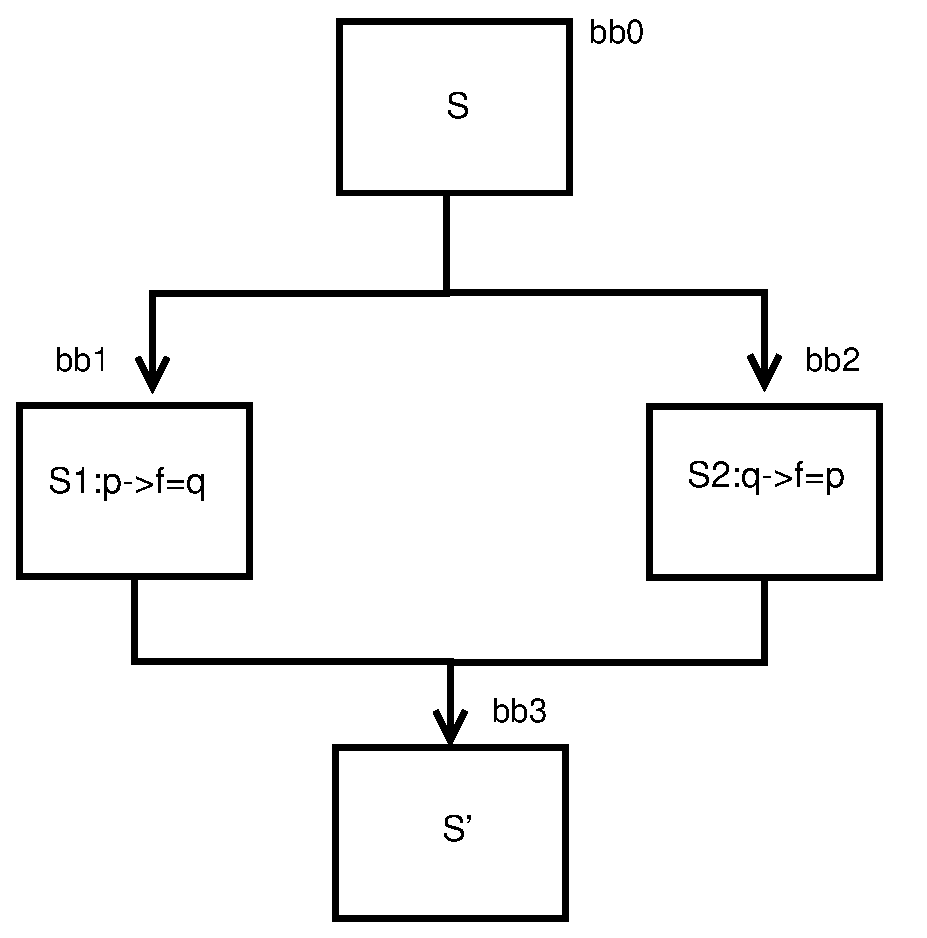
\includegraphics[scale=.35]{diagrams/Enhancements_d1.eps}
\\
\footnotesize (a)Control flow graph  \\ \\

 \scalebox{0.80}{
\begin{tabular}[h]{|l@{}|@{}c@{}|@{}c@{}|} \hline
 {\bf Basic} & $D_F$ & $I_F$ \\ 
 {\bf block} & & \\ \hline

{\tt $OUT(bb1)$} & 
\begin{tabular}{|p{3mm}|p{22mm}p{22mm}|} \hline 
            & $\p$  		& $\q$   \\ \hline
  $\p$ 	& $\epsilon$	& $\{\fieldD{f}{}\}$	 \\ \hline
  $\q$ 	& $\emptyset$	& $\epsilon$	\\ \hline
\end{tabular}
 &
\begin{tabular}{|p{3mm}|p{45mm}p{45mm}|} \hline 
            & $\p$  		& $\q$   \\ \hline
  $\p$ 	& $\{(\epsilon,\epsilon)\}$	& $\{(\fieldD{f}{}, \epsilon)\}$	 \\ \hline
  $\q$ 	& $\{(\epsilon,\fieldD{f}{}) ) \}$	& $\{(\epsilon,\epsilon)\}$	\\ \hline
\end{tabular} \\ \hline

{\tt $OUT(bb2)$} & 
\begin{tabular}{|p{3mm}|p{22mm}p{22mm}|} \hline 
            & $\p$  		& $\q$   \\ \hline
  $\p$ 	& $\epsilon$	& $\emptyset$	 \\ \hline
  $\q$ 	& $\{\fieldD{f}{}\}$ 	& $\epsilon$	\\ \hline
\end{tabular}
 &
\begin{tabular}{|p{3mm}|p{45mm}p{45mm}|} \hline 
            & $\p$  		& $\q$   \\ \hline
  $\p$ 	& $\{(\epsilon,\epsilon)\}$	& $\{ (\epsilon),\fieldD{f}{} )\}$ 	 \\ \hline
  $\q$ 	& $\{(\fieldD{f}{}, \epsilon)\}$ 	& $\{(\epsilon,\epsilon)\}$	\\ \hline
\end{tabular} \\ \hline

{\tt $IN(bb3)$} & 
\begin{tabular}{|p{3mm}|p{22mm}p{22mm}|} \hline 
            & $\p$  		& $\q$   \\ \hline
  $\p$ 	& $\epsilon$	& $\{\fieldD{f}{}\}$	 \\ \hline
  $\q$ 	& $\{\fieldD{f}{}\}$	& $\epsilon$	\\ \hline
\end{tabular}
 &
\begin{tabular}{|p{3mm}|p{45mm}p{45mm}|} \hline 
            & $\p$  		& $\q$   \\ \hline
  $\p$ 	& $\{(\epsilon,\epsilon)\}$	& $\{(\fieldD{f}{}, \epsilon),(\epsilon,\fieldD{f}{} ) \}$	 \\ \hline
  $\q$ 	& $\{(\fieldD{f}{}, \epsilon),(\epsilon,\fieldD{f}{} ) \}$	& $\{(\epsilon,\epsilon)\}$	\\ \hline
\end{tabular} \\ \hline
\end{tabular}
}
\\ \\
\footnotesize (b)Direction and Interference Matrices \\ \\

\scalebox{0.80}{
\begin{tabular}[b]{|c@{}|@{}c|}\hline
  Basic Block \  & Boolean Equations \\ \hline
 OUT(bb1) &
% \begin{tabular}{c}
$(f_{\p\q} \wedge \InC{q}) \vee (f_{\p\q} \wedge (\num{\DFM{\q}{\p}} \geq 1))$ \\ \hline

OUT(bb2) &
$(f_{\q\p} \wedge (\num{\DFM{\q}{\p}} \geq 1))$ \\ \hline

IN(bb3) & 
$((f_{\p\q} \wedge \InC{q}) \vee (f_{\p\q} \wedge (\num{\DFM{\q}{\p}} \geq 1)) \cup (f_{\q\p} \wedge (\num{\DFM{\q}{\p}} \geq 1)))$ \\ \hline
\end{tabular} 
} \\  

\footnotesize (c)Boolean equation of {\tt $p_{cycle}$}  \\
\end{tabular}
\caption{DataFlow values and CFG} \label{if-else-cfg}
\end{figure}

\textbf{Information Passed to successors: }
Here we will discuss about the less precise results that we are obtaining while passing the boolean equations to its successorss according to 
\cite{Sandeep}. Also we will discuss ways to fix this.
Let us look at the Fig:~\ref{if-else-cfg}(a), it contains a single statement in the if and else blocks.
The Direction matrices at the OUT of bb1 and bb2 are shown in Fig:~\ref{if-else-cfg}(b).
 
$f_{\p\q}$ and $f_{\q\p}$  are TRUE from basic blocks bb1 and bb2 respectively. Now if we look at the equation of {\tt $p_{cycle}$} at IN(bb3) 
from Fig:~\ref{if-else-cfg}(c) and substitute the data flow values at IN(bb3) from  Fig:~\ref{if-else-cfg}(b) we can see that it evaluates to TRUE,
inferring that the shape of \p\ as CYCLE even though its a TREE in reality. The problem here is we are not taking into consideration that only one of the 
basic blocks among bb1, bb2 will be executed.
Merging of these boolean equations does not capture that effect.

\textbf{Solution: }For this problem we propose a simple and effective solution which even reduces the memory consumption
by a good amount. What we propose is, at any statement when we evaluate a boolean equation and pass it to its successor only if that equation
evaluates to 1 otherwise we do not pass it to the successor at all. This solution works because at those basic statements which can change the heap shape,
such as $\p \rightarrow \f =\q$, whatever boolean equations are generated they alone are sufficient to determine the shape of each pointer at that program 
point.
  \begin{eqnarray*}
  S1: \q \rightarrow \g &=& \p \\
  S2: \p \rightarrow \f &=& \q   
  \end{eqnarray*}
Lets take a simple example of just two statements. 
As equations at {\tt S1} evaluates to false and hence no boolean equation is passed to {\tt S2}. It means the value of  $\InC{\p}$ for {\tt S2} 
is FALSE and $\OutC{\p}$ of {\tt S2} is same as $\GenC{\p}$ of {\tt S2}. The equation for $\GenC{\p}$, which is the same given in Fig:~\ref{if-else-cfg}(c) first row 
evaluates to TRUE hence detecting the shape correctly as a CYCLE. 

There is one case where boolean equation is to be changed to get correct results 
which is for $\GenD{p}$ of statement $\p \rightarrow \f =\q$.
\begin{eqnarray*}
	  \GenD{p}   &=&  ( f_{\p\q} \wedge (\num{\IFM{\p}{\q}} > 1) )
\end{eqnarray*}
Consider the set of statements  
\begin{eqnarray*}
  S1: \x \rightarrow \f &=& \y \\
  S2: \x \rightarrow \g &=& \y  \\
  S3: w \rightarrow \f &=& \x 
\end{eqnarray*}
After the first two statements a DAG is formed at $\x$. After the third statement a link is created from  $w$ to $\x$ via field $\f$, that means $w$ also points to a DAG. 
As the shape of $w$ before this statement was a TREE, $\InD{w}$ is empty according to the above mentioned change. We know that $\KillD{w}$ is also $\false$ for this statement, 
hence $\OutD{w}$ is nothing but $\GenD{w}$. Now consider the equation of $\GenD{w}$, it is equal to $( f_{w\x} \wedge (\num{\IFM{w}{\x}} > 1) )$. The value of 
boolean variable $f_{w\x}$ is $\true$ but value of $(\num{\IFM{w}{\x}} > 1) )$ is $\false $ as the entry $\IFM{w}{\x}$ would just contain 
$\{ \fieldD{f}{} , \epsilon \}$ . Finally evaluating the value of $\OutD{w}$ to $\false$, which is incorrect.
  
If at all we have used the old approach of passing information to successors then $\InD{w}$ would not have been empty, and would have successfully identified
the shape at $w$ as a DAG. Now to overcome this problem we have to change to the equation of $\GenD{p}$. Whenever a statement $\p \rightarrow \f = \q$ is
encountered and shape of $\q$ before this statement is a DAG, then we can simply say that $\p$ also points to a DAG. This is formalized as
\begin{eqnarray*}
	  \GenD{p}   &=&  (f_{\p\q} \wedge \InD{q}) \vee ( f_{\p\q} \wedge (\num{\IFM{\p}{\q}} > 1) )
\end{eqnarray*}

\textbf{Limitation: }This change in $\GenD{p}$ will cause loss of accuracy in one scenario (also exhibited by Ghiya et al.~\cite{Ghiya96}), but 
as a whole it has a lot of advantages in accuracy and memory consumption, so we have adopted this change. Lets look at that particular scenario.

\begin{figure}
\centering
\begin{tabular}{cc}
\begin{tabular}{c}
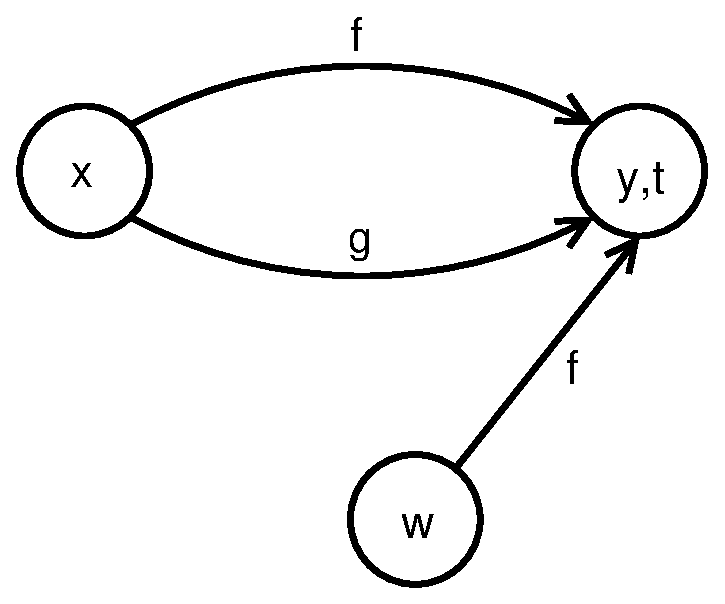
\includegraphics[scale=.4]{diagrams/Enhancements_d3.eps}
\end{tabular} & 
\begin{tabular}{c}
S1: $\x \rightarrow \f = \y$ \\
S2: $\x \rightarrow \g = \y$  \\
S3: $t = \x \rightarrow \g$ \\
S4: $w \rightarrow \f = t$
\end{tabular} \\
\footnotesize (a)Heap Graph & \footnotesize (b)Set of statements
\end{tabular}
\caption{ Example with Heap graph and Set of statements} \label{fig:enhancements_example}
\end{figure}

 
Refer to Fig:~\ref{fig:enhancements_example}, the effect of the set of statements are shown in the heap graph.
After the second statement a DAG is formed at $\x$ and when the third statement is encountered the equation of $\x$ is copied to the equation of $t$.
And at statement S4 the shape at $w$ is reported as a DAG. When this change in $\GenD{p}$ was not incorporated, the shape was reported as a TREE.
The details about how this change is making the shape vary is shown below.


(According to the original equation of $\GenD{\p}$ )

After S1: \\
$\OutD{x} = False$

After S2: \\
$\OutD{x} =  ( f_{\x\y} \wedge (\num{\IFM{\x}{\y}} > 1) )$
(which evaluates to TRUE)

After S3: \\
$\OutD{t} = ( f_{\x\y} \wedge (\num{\IFM{\x}{\y}} > 1) )$
(which evaluates to TRUE)

After S4:\\
$\OutD{w} = ( f_{wt} \wedge (\num{\IFM{w}{t}} > 1) )$ 
(which evaluates to FALSE) \\ \\
(According to the new equation of $\GenD{\p}$ )

After S4: \\
$\OutD{w} =   (f_{wt} \wedge \InD{t}) \vee ( f_{wt} \wedge (\num{\IFM{w}{t}} > 1) )$
(which evaluates to TRUE) \\

The new version of equation of $\OutD{w}$ evaluates to TRUE because of the term $\InD{t}$ which is also TRUE. As this part
was not present in the previous version of $\GenD{p}$ it correctly infers the shape of $w$ as Tree.

\section{Final Data Flow Equations}
All the modifications that were proposed are shown in  Fig:~\ref{fig:Modified Data Flow Equations}. It contains the 
final set of data flow values for each of the statements.

Let us first introduce some notations which will be used frequently in the following analysis.

$\forall \p \in \heap, \mbox{we introduce two notations } \alias{P} \mbox{ and }  \alias{p} as$ 
\begin{eqnarray*}
	\alias{P} &=& \aliasinfo{\p} \mbox{ and } \\
	\alias{p} &\in& \alias{P}
\end{eqnarray*}


\begin{figure} 
\begin{spacing}{2.0}
\begin{tabular}{|p{2.6cm}|p{12cm}|}
\hline
 {\tt p = malloc()} & 

\scalebox{0.70}{
  \begin{tabular}{lll}
	  \KillC{p}  = \InC{p} & \KillD{p} = \InD{p} &\\
	  \GenC{p} = \false  & \GenD{p} = \false &\\

	  $\forall \s \in \heap,\ \s \not= \p,$ && \\
	  $D_F^{\dkill}[\p,\s]$  =  $D_F^{\din}[\p,\s]$ & $D_F^{\dkill}[\s,\p]$  =  $D_F^{\din}[\s,\p]$ & $D_F^{\dkill}[\p,\p]$  =  $D_F^{\din}[\p,\p]$ \\
	  $D_F^{\dgen}[\p,\s]$   =  $\emptyset$         & $D_F^{\dgen}[\s,\p]$   =  $\emptyset$          &$D_F^{\dgen}[\p,\p]$   =  $\epsilonset$ \\
	  $I_F^{\dkill}[\p,\s]$  =  $I_F^{\din}[\p,\s]$ & $I_F^{\dkill}[\p,\p]$  =  $I_F^{\din}[\p,\p]$   &\\
	  $I_F^{\dgen}[\p,\s]$   =  $\emptyset$         & $I_F^{\dgen}[\p,\p]$   =  $\epsilonpairset$     &
\end{tabular}
} \\
\hline
 {\tt p = NULL} & 
\scalebox{0.70}{
  \begin{tabular}{ll}
	  \KillC{p}  = \InC{p} & \KillD{p} = \InD{p} \\
	  \GenC{p} = \false    & \GenD{p} = \false \\

	   $\forall \s \in \heap,$ & \\
	  $D_F^{\dkill}[\p,\s]$  =  $D_F^{\din}[\p,\s]$ & $D_F^{\dkill}[\s,\p]$  =  $D_F^{\din}[\s,\p]$ \\
	  $D_F^{\dgen}[\p,\s]$    =  $\emptyset$  & $D_F^{\dgen}[\s,\p]$    =  $\emptyset$ \\
	  $I_F^{\dkill}[\p,\s]$  =  $I_F^{\din}[\p,\s]$ & $I_F^{\dgen}[\p,\s]$    =  $\emptyset$ 
  \end{tabular}
} \\
\hline
\begin{tabular}{l}
{\tt p = q} \\
{\tt p =\&(q$\rightarrow$f)} \\
{\tt p = q op n}
\end{tabular}
 &
\scalebox{0.70}{
\begin{tabular}{l}

	\KillC{p} = \InC{p} \quad\qquad \KillD{p} = \InD{p} \\ 
	\GenC{p}   = \InC{q}[q/p] \quad \GenD{p} = \InD{q}[q/p] \\ 
	where $X[\q / \p]$ creates a copy of $X$ with all occurrences
	of $\q$ replaced by $\p$.\\

      $\forall \s \in \heap,  \s \not= \p,  \forall f \in \fields,$ \\

	$f_{\p\s} = f_{\q\s}$  \quad  $f_{\s\p} = f_{\s\q}$ \\
	$D_F^{\dkill}[\p, \s]$  =  $D_F^{\din}[\p, \s]$ \quad $D_F^{\dkill}[\s, \p]$  =  $D_F^{\din}[\s, \p]$ \quad $D_F^{\dkill}[\p, \p]$  =  $D_F^{\din}[\p, \p]$ \\
	$D_F^{\dgen}[\p, \s]$    =  $D_F^{\din}[\q, \s]$ \quad $D_F^{\dgen}[\s, \p]$    =  $D_F^{\din}[\s, \q]$ \quad $D_F^{\dgen}[\p, \p]$    =  $D_F^{\din}[\q, \q]$  \\
	$I_F^{\dkill}[\p, \s]$  =  $I_F^{\din}[\p, \s]$ \qquad $I_F^{\dgen}[\p, \s]$    =   $I_F^{\din}[\q, \s]$ \\
	$I_F^{\dkill}[\p, \p]$  =  $I_F^{\din}[\p, \p]$ \qquad $I_F^{\dgen}[\p, \p]$    = $I_F^{\din}[\q, \q]$ 
  \end{tabular}
} \\
\hline
\tt{ $\delta$ = p }
&
\scalebox{0.70}{
    \begin{tabular}{l}
	$\GenC{\delta}   = \InC{\p}[\p/\delta] \qquad\qquad \GenD{\delta} = \InD{\p}[\p/\delta]$ \\
	$\forall \s \in \heap, \s \not= \p, \forall f \in \fields$ \\
	$\KillC{\s} = \InC{\s}  \qquad\qquad\qquad  \KillC{\s} = \InD{\s}$  \\
	$\GenC{\s}  = \InC{\s}[\p/\delta] \qquad\qquad   \GenD{\s} = \InD{\s}[\p/\delta]$ \\ 	 
	where $X[\q / \p]$ creates a copy of $X$ with all occurrences
	of $\q$ replaced by $\p$. \\
	$\forall \s \in \heap, \s \not= \p, \forall f \in \fields$ \\
	$f_{\delta\s} = f_{\p\s}$  \quad  $f_{\s\delta} = f_{\s\p}$ \\
	$D_F^{\dgen}[\delta,\s]$    =  $D_F^{\din}[\p,\s]$ \quad  $D_F^{\dgen}[\s,\delta]$    =  $D_F^{\din}[\s,\p]$ \quad  
		 $D_F^{\dgen}[\delta,\delta]$    =  $D_F^{\din}[\p,\p]$  \\
	 $I_F^{\dgen}[\delta,\s]$    =   $I_F^{\din}[\p,\s]$ \quad \; $I_F^{\dgen}[\delta,\delta]$    = $I_F^{\din}[\p,\p]$  \\  
    \end{tabular}
} \\
\hline
\end{tabular}
\end{spacing}
\end{figure}

\begin{figure}[p]
\begin{spacing}{2.0}
\begin{tabular}{|p{2.6cm}|p{12cm}|}
\hline
{\tt p$\rightarrow$f=null}
&
	\scalebox{0.70}{
	  \begin{tabular}{l}
	  \KillC{p}  = \false, \quad \KillD{p} = \false \\
	  \GenC{p} = \false, \quad \GenD{p} = \false  \\
		$\forall \q,\s \in \heap, \s \notin \alias{P}$ \\
	  $f_{\alias{p}\q}$ = \false \\
	  $D_F^{\dkill}[\alias{p}, \q]$  = $\project{D_F^{\din}[\p, \q]}{f}$ \qquad  \;  ${D_{F}^{{\dkill}}[\s, \q]}  = \emptyset  $  \\
 	  $I_F^{\dkill}[\alias{p}, \s] = \{(\alpha,  \beta) \ \vert\ (\alpha, \beta) \in I_F^{\din}[\p,  \q] \mbox, \ \alpha \equiv f^\anysup \}$ \\ 
 	  ${I_F^{\dkill}[\q, \s]} = \emptyset \mbox{ if } \q \notin \alias{P}$ \qquad\qquad   
 	  ${I_F^{\dkill}[\alias{p}, \alias{p}]} = \{(\alpha,  \beta) \ \vert\ (\alpha, \beta) \in I_F^{\din}[\p,  \p] \mbox, \ \alpha \equiv f^\anysup \}$
  \end{tabular}
} \\
\hline
{\tt p$\rightarrow$f = q}
&
    \scalebox{0.70}{
    \begin{tabular}{l}
	  \mbox{The KILL relations are same as that of {\tt p$\rightarrow$f = null}} \\
	  $\GenC{\p}   =  (f_{\p\q} \wedge \InC{q}) \vee (f_{\p\q} \wedge (\num{\DFM{\q}{\p}} \geq 1))$  \quad 
	  $\GenD{p}   =  (f_{\p\q} \wedge \InD{q}) \vee ( f_{\p\q} \wedge (\num{\IFM{\p}{\q}} > 1) )$ \\
 	  $\GenC{q}   = f_{\p\q} \wedge (\num{\DFM{\q}{\p}} \geq 1)$ \quad\qquad\qquad\qquad\quad $\GenD{q} = \false$\\ 
	  $f_{\alias{p}\alias{q}} = \true$ \\
%-------------------------------------------------------Newly Added-----------------------------------------------------------------------------

%	 $\GenC{\x}   =  \GenC{\p}[\p/\x] \qquad\qquad \GenD{\x} = \GenD{\p}[\p/\x]\ \forall \x \in \alias{P}$\\
%	 $\GenC{\x}   =  \GenC{\q}[\q/\x] \qquad\qquad \GenD{\x} = \GenD{\q}[\q/\x]\ \forall \x \in \alias{Q}$\\

% DO NOT DELETE
%The above rule said that if x alias to p then create a similar eqn for x. But there might be cases like x alias to p and also to q but p and q are not
%aliases. Like
% if{x = p} else {x=q}  p->f = q; Here the corresponding eqn will be x(c) = f(xq) and D[qx]>=1 whih will be true but inreality x is not cycle.
% this is mitigates by the below eqns.

	  $\GenC{\s} =  ((\num{\DFM{\s}{\p}} \geq 1) \wedge f_{\p\q} \wedge \InC{q})$ $\vee\ ((\num{\DFM{\s}{\p}} \geq 1) \wedge f_{\p\q} \wedge
 	  (\num{\DFM{\q}{\p}} \geq 1))$ \\ 
	  \quad  $\vee\ ((\num{\DFM{\s}{\q}} \geq 1) \wedge f_{\p\q}
	  \wedge (\num{\DFM{\q}{\p}} \geq 1))$, \ \   $\forall \s \in \heap, \s \not= p,q $\\
	  $\GenD{\s}   = (\num{\DFM{\s}{\p}} \geq 1) \wedge
	  f_{\p\q} \wedge (\num{\IFM{\s}{\q}} > 1)$, \ $\forall \s \in \heap, \s \not= p,q $\\


%-----------------------------------------------------------------------------------------------------------------------------------------
% 	 $ D_F^{\dgen}[\myr, \s] = \num{D_F^{\din}[\q, \s]} \star              %modified as
% 	  D_F^{\din}[\myr, \p],\ \s \not= \p,\ \myr \not\in
% 	  \{\p, \q\} $\\ 	

 $ D_F^{\dgen}[\myr, \s] = \num{D_F^{\din}[\q, \s]} \star  D_F^{\din}[\myr, \p],\ \s \notin \alias{P},\ \myr \notin \alias{P},\ \myr \notin \alias{Q}$ \\
%-----------------------------------------------------------------------------------------------------------------------------------------
	  $D_F^{\dgen}[\myr, \alias{p}] = \num{D_F^{\din}[\q,\p]} \star D_F^{\din}[\myr, \p], \ \myr \notin \alias{P}$\\
	  $D_F^{\dgen}[\alias{p}, \myr] = \num{D_F^{\din}[\q, \myr]} \star (\remOne{D_F^{\din}[\p, \p]}{\epsilonset} \cup \{f^{\indrct 1}\})$, \ \  $\myr \notin \alias{Q}$ \\ 
	  $D_F^{\dgen}[\alias{p}, \alias{q}] = \{\fieldD{f}{}\}\ \cup\ (\num{D_F^{\din}[\q, \q] - \epsilonset} \star \{\fieldI{f}{}{1}\})\ \cup\ (\num{D_F^{\din}[\q, \q]} \star ( \remOne{D_F^{\din}[\p, \p]}{\{\project{D_F^{\din}[\p,\p]}{f} \cup \epsilonset \}}))$ \\ 
	  $D_F^{\dgen}[\alias{q}, \alias{q}] = 1 \star D_F^{\din}[\q, \p]$ \\
	  $D_F^{\dgen}[\alias{q}, \myr] = \num{D_F^{\din}[\q, \myr]} \star D_F^{\din}[\q, \p],\ \myr \notin \alias{P},\ \myr \notin \alias{Q}$ \\ 
%-----------------------------------------------------------------------------------------------------------------------------------------
% 	  $I_F^{\dgen}[\p, \q] = \{(\fieldD{f}{}, \epsilon)\}                   %modified as
% 	  \cup ((1 \star (\remOne{D_F^{\din}[\p,
% 	      \p]}{\epsilonset})) \times \epsilonset)$ \\
	  
	  $I_F^{\dgen}[\alias{p}, \alias{q}] = \{(\fieldD{f}{}, \epsilon)\}
	  \cup ((1 \star (\remOne{D_F^{\din}[\p,
      \p]}{ \{\project{D_F^{\din}[\p,\p]}{f} \cup \epsilonset \} })) \times \epsilonset) \cup  \I$ \\
 	  \quad \quad where \ 
 	  $\I  =   \bigcup_{\x\in\heap,\x \notin \alias{P},\alias{Q} } \{ {D_F^{\din}[\p,\x] \times D_F^{\din}[\q,\x] \ \vert \  \ \num{D_F^{\din}[\p,\x]} >1 , \num{D_F^{\din}[\q,\x]} >1} \}$ \\
%-----------------------------------------------------------------------------------------------------------------------------------------
	  
	  $I_F^{\dgen}[\alias{p}, \myr]$ = 
 	  $(1 \star (\remOne{D_F^{\din}[\p, \p]}{\epsilonset})) \times 
	  \{\beta\ \vert\ (\alpha, \beta) \in I_F^{\din}[\q, \myr] \}$  
	  $\cup\ \{f^\drct\} \times 
	  \{\beta\ \vert\ (\epsilon, \beta) \in I_F^{\din}[\q, \myr] \}$ \\
	  \quad \quad  $\cup\ \{f^{\indrct 1}\} \times 
	   \{\beta\ \vert\ (\alpha, \beta) \in I_F^{\din}[\q, \myr],
	  \alpha \not= \epsilon \}$, 
	  $\qquad \qquad \myr \notin \alias{P}, \alias{Q}$ \\


%-----------------------------------------------------------------------------------------------------------------------------------------
% 	  $I_F^{\dgen}[\s, \q] = (1 \star D_F^{\din}[\s, \p]) \times   %modified as
% 	  \epsilonset,\ \s \not\in \{\p, \q\}$ \\
	  
 	  $I_F^{\dgen}[\s, \alias{q}] = (1 \star D_F^{\din}[\s, \p]) \times 
 	  \epsilonset,\ \s \notin \alias{P},\ \alias{Q}$ \\

%-----------------------------------------------------------------------------------------------------------------------------------------

 %-----------------------------------------------------------------------------------------------------------------------------------------
% 	  $I_F^{\dgen}[\s, \myr] = (1 \star D_F^{\din}[\s, \p])           % modified as
% 	  \times \{\beta\ \vert\ (\alpha, \beta) \in I_F^{\din}[\q,
%  	    \myr]\}$,
% 	    $ \qquad \s \not\in \{\p, \q\},\ \myr \not\in \{\p,
% 	  \q\},\ \s \not= \myr$

 	  $I_F^{\dgen}[\s, \myr] = (1 \star D_F^{\din}[\s, \p])           % modified as
 	  \times \{\beta\ \vert\ (\alpha, \beta) \in I_F^{\din}[\q,
  	    \myr]\}$,
 	    $ \qquad \s \not\in \alias{P},\alias{Q},\ \myr \not\in \alias{P},\alias{Q},\ \s \not= \myr$ \\
  \end{tabular}
 }  \\
\hline
\end{tabular}
\end{spacing}
\end{figure} 



\begin{figure}[p]
\begin{spacing}{2.0}
\begin{tabular}{|p{2.6cm}|p{12cm}|}
\hline
{\tt p = q$\rightarrow$f} &
    \scalebox{0.70}{
    \begin{tabular}{l}
	The KILL relations are same as that of {\tt p = NULL} \\
	$\GenC{p} = \InC{q} \qquad \GenD{p} = \InD{q}$ \\

	$f_{\alias{q}\p} = \true$ \quad
	${h_{\p\myr}} =
	\num{\project{D_F^{\din}[\q,\myr]}{f}} \geq 1\quad
	\forall h \in \fields, \forall \myr \in \heap$  \\

	$ \upath \quad=\quad \epsilonset \cup \ \bigcup_{f\in\fields} \{f^{\drct},
	f^{\indrct\infty}\}$  \\ \\

	$\forall \s \in \heap, \s \not=\p$ \\
	$D_1[\p, \s] =  \left\{\begin{array}{@{}ll}
	                        \upath & \{ \project{D_F^{\din}[\q, \s]}{f} - f^{\drct} \} \not= \emptyset \\
				\{ \epsilon \} & \project{D_F^{\din}[\q, \s]}{f} = f^{\drct}
	                       \end{array}\right.$
	\quad
	$D_1[\p, \p] = \left \{ \begin{array}{@{}ll}
	  \upath& \q.\shape \mbox{ evaluates to } \Cycle \\
	  \epsilonset & \mbox{Otherwise}
	\end{array}. \right. $  \\
	$I_1[\p, \p] = \upath \times \upath $ \\ \\

%-----------------------------------------------------------------------------------------------------------------------------------------
% 	${D_2[\q,\p]} = \{ f^{\drct}\} \cup (\infty \star (\remOne{D_F^{\din}[\q, \q]}{\epsilonset})) \cup \upath$  \\   modified as
	${D_2[\alias{q},\p]} = \left\{\begin{array}{@{}ll}
	f^{\drct} & q_{in}^{tree}=\true \\
	\{ f^{\drct}\} \cup (\infty \star (\remOne{D_F^{\din}[\q, \q]}{\epsilonset})) \cup \upath &  \mbox{Otherwise} 
	\end{array}\right.$  \ \  $if \q \not = \p$ \\ 

  $D_2[\s, \p] = \infty \star D_F^{\din}[\s, \q]$ \quad $\forall \s \in \heap, \s \notin \alias{Q},\ \s \not=\p$ \\

	$I_2[\s, \p] = D_2[\s, \p] \times \epsilonset \quad \forall \s \in \heap $	\\ \\


	$D_3[\s, \p] = \{ \alpha \ \vert \ (f^{\drct}, \alpha) \in I_F^{\din}[\q, \s] \}$  \\
	$I_3[\s, \p] = \{\alpha \ \vert\ (f^\anysup, \alpha) \in I_F^{\din}[\q, \s]\} \times \upath$ \\ \\

	Final $I_F$ and $D_F$ relations are: \\

	$D_F^{\dgen}[\myr, \s] =  D_1[\myr, \s] \cup D_2[\myr, \s] \cup D_3[\myr, \s] \quad \forall\myr,\s \in \heap$  \\
	$I_F^{\dgen}[\myr, \s] =  I_1[\myr, \s] \cup I_2[\myr, \s] \cup I_3[\myr, \s] \quad \forall\myr,\s \in \heap$   \\
    \end{tabular}
  } \\
\hline

\end{tabular}
\end{spacing}
\caption{Modified Data Flow Equations}  \label{fig:Modified Data Flow Equations}
\end{figure} 

